\documentclass[twoside]{book}

% Packages required by doxygen
\usepackage{fixltx2e}
\usepackage{calc}
\usepackage{doxygen}
\usepackage[export]{adjustbox} % also loads graphicx
\usepackage{graphicx}
\usepackage[utf8]{inputenc}
\usepackage{makeidx}
\usepackage{multicol}
\usepackage{multirow}
\PassOptionsToPackage{warn}{textcomp}
\usepackage{textcomp}
\usepackage[nointegrals]{wasysym}
\usepackage[table]{xcolor}

% Font selection
\usepackage[T1]{fontenc}
\usepackage[scaled=.90]{helvet}
\usepackage{courier}
\usepackage{amssymb}
\usepackage{sectsty}
\renewcommand{\familydefault}{\sfdefault}
\allsectionsfont{%
  \fontseries{bc}\selectfont%
  \color{darkgray}%
}
\renewcommand{\DoxyLabelFont}{%
  \fontseries{bc}\selectfont%
  \color{darkgray}%
}
\newcommand{\+}{\discretionary{\mbox{\scriptsize$\hookleftarrow$}}{}{}}

% Page & text layout
\usepackage{geometry}
\geometry{%
  a4paper,%
  top=2.5cm,%
  bottom=2.5cm,%
  left=2.5cm,%
  right=2.5cm%
}
\tolerance=750
\hfuzz=15pt
\hbadness=750
\setlength{\emergencystretch}{15pt}
\setlength{\parindent}{0cm}
\setlength{\parskip}{3ex plus 2ex minus 2ex}
\makeatletter
\renewcommand{\paragraph}{%
  \@startsection{paragraph}{4}{0ex}{-1.0ex}{1.0ex}{%
    \normalfont\normalsize\bfseries\SS@parafont%
  }%
}
\renewcommand{\subparagraph}{%
  \@startsection{subparagraph}{5}{0ex}{-1.0ex}{1.0ex}{%
    \normalfont\normalsize\bfseries\SS@subparafont%
  }%
}
\makeatother

% Headers & footers
\usepackage{fancyhdr}
\pagestyle{fancyplain}
\fancyhead[LE]{\fancyplain{}{\bfseries\thepage}}
\fancyhead[CE]{\fancyplain{}{}}
\fancyhead[RE]{\fancyplain{}{\bfseries\leftmark}}
\fancyhead[LO]{\fancyplain{}{\bfseries\rightmark}}
\fancyhead[CO]{\fancyplain{}{}}
\fancyhead[RO]{\fancyplain{}{\bfseries\thepage}}
\fancyfoot[LE]{\fancyplain{}{}}
\fancyfoot[CE]{\fancyplain{}{}}
\fancyfoot[RE]{\fancyplain{}{\bfseries\scriptsize Generated by Doxygen }}
\fancyfoot[LO]{\fancyplain{}{\bfseries\scriptsize Generated by Doxygen }}
\fancyfoot[CO]{\fancyplain{}{}}
\fancyfoot[RO]{\fancyplain{}{}}
\renewcommand{\footrulewidth}{0.4pt}
\renewcommand{\chaptermark}[1]{%
  \markboth{#1}{}%
}
\renewcommand{\sectionmark}[1]{%
  \markright{\thesection\ #1}%
}

% Indices & bibliography
\usepackage{natbib}
\usepackage[titles]{tocloft}
\setcounter{tocdepth}{3}
\setcounter{secnumdepth}{5}
\makeindex

% Hyperlinks (required, but should be loaded last)
\usepackage{ifpdf}
\ifpdf
  \usepackage[pdftex,pagebackref=true]{hyperref}
\else
  \usepackage[ps2pdf,pagebackref=true]{hyperref}
\fi
\hypersetup{%
  colorlinks=true,%
  linkcolor=blue,%
  citecolor=blue,%
  unicode%
}

% Custom commands
\newcommand{\clearemptydoublepage}{%
  \newpage{\pagestyle{empty}\cleardoublepage}%
}

\usepackage{caption}
\captionsetup{labelsep=space,justification=centering,font={bf},singlelinecheck=off,skip=4pt,position=top}

%===== C O N T E N T S =====

\begin{document}

% Titlepage & ToC
\hypersetup{pageanchor=false,
             bookmarksnumbered=true,
             pdfencoding=unicode
            }
\pagenumbering{roman}
\begin{titlepage}
\vspace*{7cm}
\begin{center}%
{\Large Yay A Mouse }\\
\vspace*{1cm}
{\large Generated by Doxygen 1.8.11}\\
\end{center}
\end{titlepage}
\clearemptydoublepage
\tableofcontents
\clearemptydoublepage
\pagenumbering{arabic}
\hypersetup{pageanchor=true}

%--- Begin generated contents ---
\chapter{Hierarchical Index}
\section{Class Hierarchy}
This inheritance list is sorted roughly, but not completely, alphabetically\+:\begin{DoxyCompactList}
\item Mono\+Behaviour\begin{DoxyCompactList}
\item \contentsline{section}{Camera\+Controller}{\pageref{class_camera_controller}}{}
\item \contentsline{section}{Food}{\pageref{class_food}}{}
\item \contentsline{section}{Food\+Controller}{\pageref{class_food_controller}}{}
\item \contentsline{section}{Mouse}{\pageref{class_mouse}}{}
\item \contentsline{section}{Object\+Pool}{\pageref{class_object_pool}}{}
\item \contentsline{section}{Pool\+Member}{\pageref{class_pool_member}}{}
\item \contentsline{section}{Touch\+Test}{\pageref{class_touch_test}}{}
\end{DoxyCompactList}
\end{DoxyCompactList}

\chapter{Class Index}
\section{Class List}
Here are the classes, structs, unions and interfaces with brief descriptions\+:\begin{DoxyCompactList}
\item\contentsline{section}{\hyperlink{class_abilities}{Abilities} \\*Container class for a player\textquotesingle{}s abilities at any point in time. Always associated with a Player instance. }{\pageref{class_abilities}}{}
\item\contentsline{section}{\hyperlink{class_ability}{Ability} \\*Base class to where all abilities with a Happiness cost and limited duration are derived from }{\pageref{class_ability}}{}
\item\contentsline{section}{\hyperlink{class_ability_controller}{Ability\+Controller} \\*Script class to encapsulate mouse ability logic. Implements functions to be called when abilities are activated by a player or when a player is affected by an ability activated by another player. }{\pageref{class_ability_controller}}{}
\item\contentsline{section}{\hyperlink{class_ability_controls}{Ability\+Controls} }{\pageref{class_ability_controls}}{}
\item\contentsline{section}{\hyperlink{class_beastly_buffet}{Beastly\+Buffet} \\*A player\textquotesingle{}s Beastly Buffet ability. }{\pageref{class_beastly_buffet}}{}
\item\contentsline{section}{\hyperlink{class_camera_controller}{Camera\+Controller} \\*Script for controlling camera behavior Stores global screen info such as the default aspect ratio, pixels per unit, and min. and max. x and y coordinates in Unity units Camera viewport adapts to device screen size and introduces pillarboxing/letterboxing to maintain the correct aspect ratio }{\pageref{class_camera_controller}}{}
\item\contentsline{section}{\hyperlink{class_fat_mouse}{Fat\+Mouse} \\*A player\textquotesingle{}s Fat \hyperlink{class_mouse}{Mouse} ability. }{\pageref{class_fat_mouse}}{}
\item\contentsline{section}{\hyperlink{class_fearless}{Fearless} \\*A player\textquotesingle{}s \hyperlink{class_fearless}{Fearless} ability. }{\pageref{class_fearless}}{}
\item\contentsline{section}{\hyperlink{class_food}{Food} }{\pageref{class_food}}{}
\item\contentsline{section}{\hyperlink{class_food_controller}{Food\+Controller} \\*Script attached to \hyperlink{class_food_controller}{Food\+Controller} object that controls behavior such as food spawning, and food movement. }{\pageref{class_food_controller}}{}
\item\contentsline{section}{\hyperlink{class_immunity}{Immunity} \\*A player\textquotesingle{}s \hyperlink{class_immunity}{Immunity} ability. }{\pageref{class_immunity}}{}
\item\contentsline{section}{\hyperlink{class_level_controller}{Level\+Controller} \\*Handles game state, such as the player\textquotesingle{}s combo streak, whether or not the player is in frenzy feeding mode, and the number of players in a game. Handles state of combo and player avatar UI as well (?) }{\pageref{class_level_controller}}{}
\item\contentsline{section}{\hyperlink{class_mouse}{Mouse} \\*Script class that controls behaviour of the mouse. Keeps track of mouses status such as weight, happiness, level, and attributes that can be set by player abilities\+: (immunity, leptin\+Deficiency, fearless) }{\pageref{class_mouse}}{}
\item\contentsline{section}{\hyperlink{class_object_pool}{Object\+Pool} \\*Generic class for handling object pooling. The type of game object to pool can be specified by assigning the public member obj in the inspector panel. Keeps track of active objects in the pool. Has methods to get object from pool and return object to the pool. Pool is maintained as a list and can grow dynamically. }{\pageref{class_object_pool}}{}
\item\contentsline{section}{\hyperlink{class_assets_1_1_scripts_1_1_player}{Assets.\+Scripts.\+Player} \\*Class to contain player specific data, currently only contains the player\textquotesingle{}s \hyperlink{class_abilities}{Abilities}. }{\pageref{class_assets_1_1_scripts_1_1_player}}{}
\item\contentsline{section}{\hyperlink{class_pool_member}{Pool\+Member} \\*Script that is attached to members of an object pool when they are first instantiated. Allows object to keep track of the pool they belong to and be deactivated and returned to that pool. }{\pageref{class_pool_member}}{}
\item\contentsline{section}{\hyperlink{class_scary_cat}{Scary\+Cat} \\*A player\textquotesingle{}s Scary Cat ability. }{\pageref{class_scary_cat}}{}
\item\contentsline{section}{\hyperlink{class_thief}{Thief} \\*A player\textquotesingle{}s \hyperlink{class_thief}{Thief} ability. }{\pageref{class_thief}}{}
\item\contentsline{section}{\hyperlink{class_touch_test}{Touch\+Test} }{\pageref{class_touch_test}}{}
\item\contentsline{section}{\hyperlink{class_treats_galore}{Treats\+Galore} \\*A player\textquotesingle{}s Treats Galore ability. }{\pageref{class_treats_galore}}{}
\end{DoxyCompactList}

\chapter{Class Documentation}
\hypertarget{class_camera_controller}{}\section{Camera\+Controller Class Reference}
\label{class_camera_controller}\index{Camera\+Controller@{Camera\+Controller}}


Script for controlling camera behavior Stores global screen info such as the default aspect ratio, pixels per unit, and min. and max. x and y coordinates in Unity units Camera viewport adapts to device screen size and introduces pillarboxing/letterboxing to maintain the correct aspect ratio  


Inheritance diagram for Camera\+Controller\+:\begin{figure}[H]
\begin{center}
\leavevmode
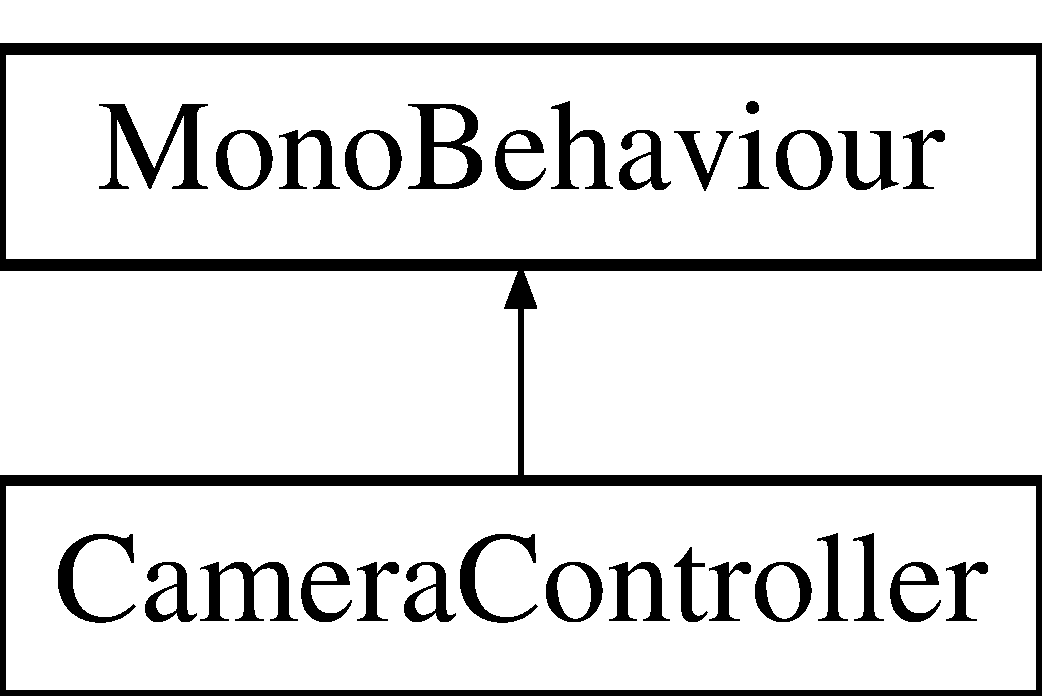
\includegraphics[height=2.000000cm]{class_camera_controller}
\end{center}
\end{figure}
\subsection*{Static Public Attributes}
\begin{DoxyCompactItemize}
\item 
static float \hyperlink{class_camera_controller_a382108f331b87cc67e6694cde84b3910}{Pixels\+Per\+Unit}
\begin{DoxyCompactList}\small\item\em Pixels per unit, for referencing in other scripts \end{DoxyCompactList}\item 
static float \hyperlink{class_camera_controller_afbf830e2978734f35fb745fd63d13ca4}{Min\+X\+Units}
\begin{DoxyCompactList}\small\item\em Smallest x coordinate, in Unity units, that fits into the screen \end{DoxyCompactList}\item 
static float \hyperlink{class_camera_controller_a6b97db2514a3f59c74eb56a013e00c85}{Max\+X\+Units}
\begin{DoxyCompactList}\small\item\em Largest x coordinate, in Unity units, that fits into the screen \end{DoxyCompactList}\item 
static float \hyperlink{class_camera_controller_a66577648bab85619c6e72059e0ac4029}{Min\+Y\+Units}
\begin{DoxyCompactList}\small\item\em Smallest y coordinate, in Unity units, that fits into the screen \end{DoxyCompactList}\item 
static float \hyperlink{class_camera_controller_a1467ca3823ce8566582bcb6a37d19913}{Max\+Y\+Units}
\begin{DoxyCompactList}\small\item\em Largest y coordinate, in Unity units, that fits into the screen \end{DoxyCompactList}\end{DoxyCompactItemize}


\subsection{Detailed Description}
Script for controlling camera behavior Stores global screen info such as the default aspect ratio, pixels per unit, and min. and max. x and y coordinates in Unity units Camera viewport adapts to device screen size and introduces pillarboxing/letterboxing to maintain the correct aspect ratio 



\subsection{Member Data Documentation}
\index{Camera\+Controller@{Camera\+Controller}!Max\+X\+Units@{Max\+X\+Units}}
\index{Max\+X\+Units@{Max\+X\+Units}!Camera\+Controller@{Camera\+Controller}}
\subsubsection[{\texorpdfstring{Max\+X\+Units}{MaxXUnits}}]{\setlength{\rightskip}{0pt plus 5cm}float Camera\+Controller.\+Max\+X\+Units\hspace{0.3cm}{\ttfamily [static]}}\hypertarget{class_camera_controller_a6b97db2514a3f59c74eb56a013e00c85}{}\label{class_camera_controller_a6b97db2514a3f59c74eb56a013e00c85}


Largest x coordinate, in Unity units, that fits into the screen 

\index{Camera\+Controller@{Camera\+Controller}!Max\+Y\+Units@{Max\+Y\+Units}}
\index{Max\+Y\+Units@{Max\+Y\+Units}!Camera\+Controller@{Camera\+Controller}}
\subsubsection[{\texorpdfstring{Max\+Y\+Units}{MaxYUnits}}]{\setlength{\rightskip}{0pt plus 5cm}float Camera\+Controller.\+Max\+Y\+Units\hspace{0.3cm}{\ttfamily [static]}}\hypertarget{class_camera_controller_a1467ca3823ce8566582bcb6a37d19913}{}\label{class_camera_controller_a1467ca3823ce8566582bcb6a37d19913}


Largest y coordinate, in Unity units, that fits into the screen 

\index{Camera\+Controller@{Camera\+Controller}!Min\+X\+Units@{Min\+X\+Units}}
\index{Min\+X\+Units@{Min\+X\+Units}!Camera\+Controller@{Camera\+Controller}}
\subsubsection[{\texorpdfstring{Min\+X\+Units}{MinXUnits}}]{\setlength{\rightskip}{0pt plus 5cm}float Camera\+Controller.\+Min\+X\+Units\hspace{0.3cm}{\ttfamily [static]}}\hypertarget{class_camera_controller_afbf830e2978734f35fb745fd63d13ca4}{}\label{class_camera_controller_afbf830e2978734f35fb745fd63d13ca4}


Smallest x coordinate, in Unity units, that fits into the screen 

\index{Camera\+Controller@{Camera\+Controller}!Min\+Y\+Units@{Min\+Y\+Units}}
\index{Min\+Y\+Units@{Min\+Y\+Units}!Camera\+Controller@{Camera\+Controller}}
\subsubsection[{\texorpdfstring{Min\+Y\+Units}{MinYUnits}}]{\setlength{\rightskip}{0pt plus 5cm}float Camera\+Controller.\+Min\+Y\+Units\hspace{0.3cm}{\ttfamily [static]}}\hypertarget{class_camera_controller_a66577648bab85619c6e72059e0ac4029}{}\label{class_camera_controller_a66577648bab85619c6e72059e0ac4029}


Smallest y coordinate, in Unity units, that fits into the screen 

\index{Camera\+Controller@{Camera\+Controller}!Pixels\+Per\+Unit@{Pixels\+Per\+Unit}}
\index{Pixels\+Per\+Unit@{Pixels\+Per\+Unit}!Camera\+Controller@{Camera\+Controller}}
\subsubsection[{\texorpdfstring{Pixels\+Per\+Unit}{PixelsPerUnit}}]{\setlength{\rightskip}{0pt plus 5cm}float Camera\+Controller.\+Pixels\+Per\+Unit\hspace{0.3cm}{\ttfamily [static]}}\hypertarget{class_camera_controller_a382108f331b87cc67e6694cde84b3910}{}\label{class_camera_controller_a382108f331b87cc67e6694cde84b3910}


Pixels per unit, for referencing in other scripts 



The documentation for this class was generated from the following file\+:\begin{DoxyCompactItemize}
\item 
Assets/\+Scripts/Camera\+Controller.\+cs\end{DoxyCompactItemize}

\hypertarget{class_food}{}\section{Food Class Reference}
\label{class_food}\index{Food@{Food}}
Inheritance diagram for Food\+:\begin{figure}[H]
\begin{center}
\leavevmode
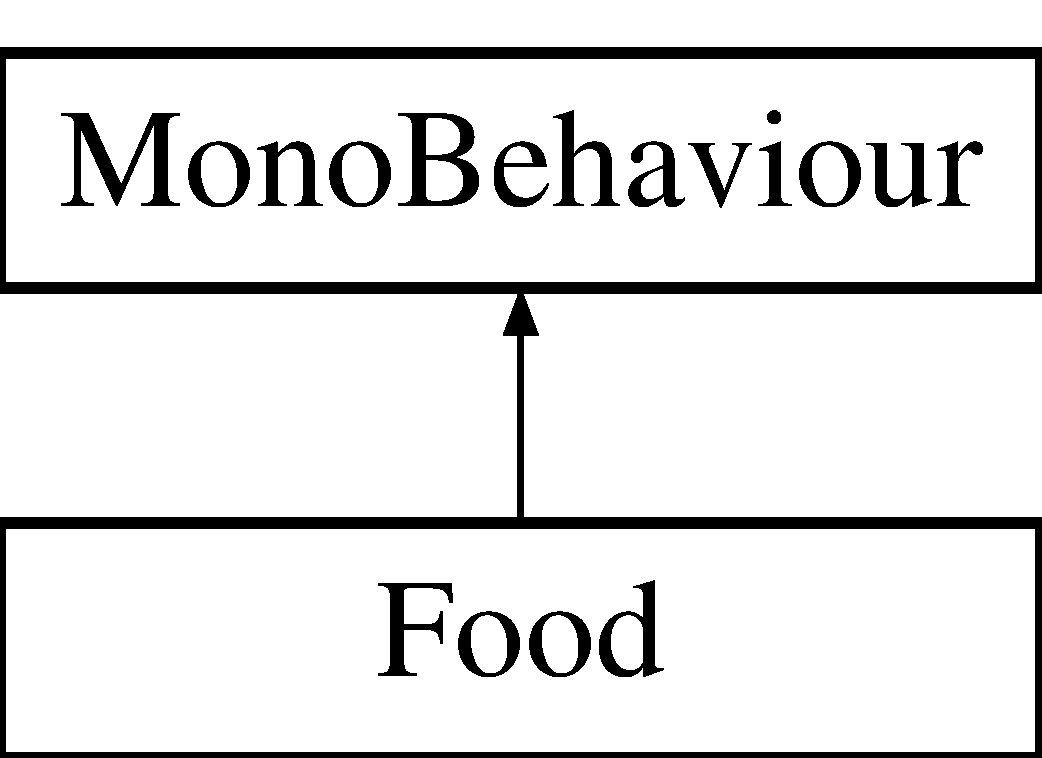
\includegraphics[height=2.000000cm]{class_food}
\end{center}
\end{figure}
\subsection*{Public Attributes}
\begin{DoxyCompactItemize}
\item 
int {\bfseries value} = 5\hypertarget{class_food_a54e3f74b4f899a29275846610db2f6ef}{}\label{class_food_a54e3f74b4f899a29275846610db2f6ef}

\item 
string {\bfseries type} = \char`\"{}Normal\char`\"{}\hypertarget{class_food_adff3b58565023eaa590bc565163b5be8}{}\label{class_food_adff3b58565023eaa590bc565163b5be8}

\end{DoxyCompactItemize}


The documentation for this class was generated from the following file\+:\begin{DoxyCompactItemize}
\item 
Assets/\+Scripts/Food.\+cs\end{DoxyCompactItemize}

\hypertarget{class_food_controller}{}\section{Food\+Controller Class Reference}
\label{class_food_controller}\index{Food\+Controller@{Food\+Controller}}


Script attached to \hyperlink{class_food_controller}{Food\+Controller} object that controls behavior such as food spawning, and food movement.  


Inheritance diagram for Food\+Controller\+:\begin{figure}[H]
\begin{center}
\leavevmode
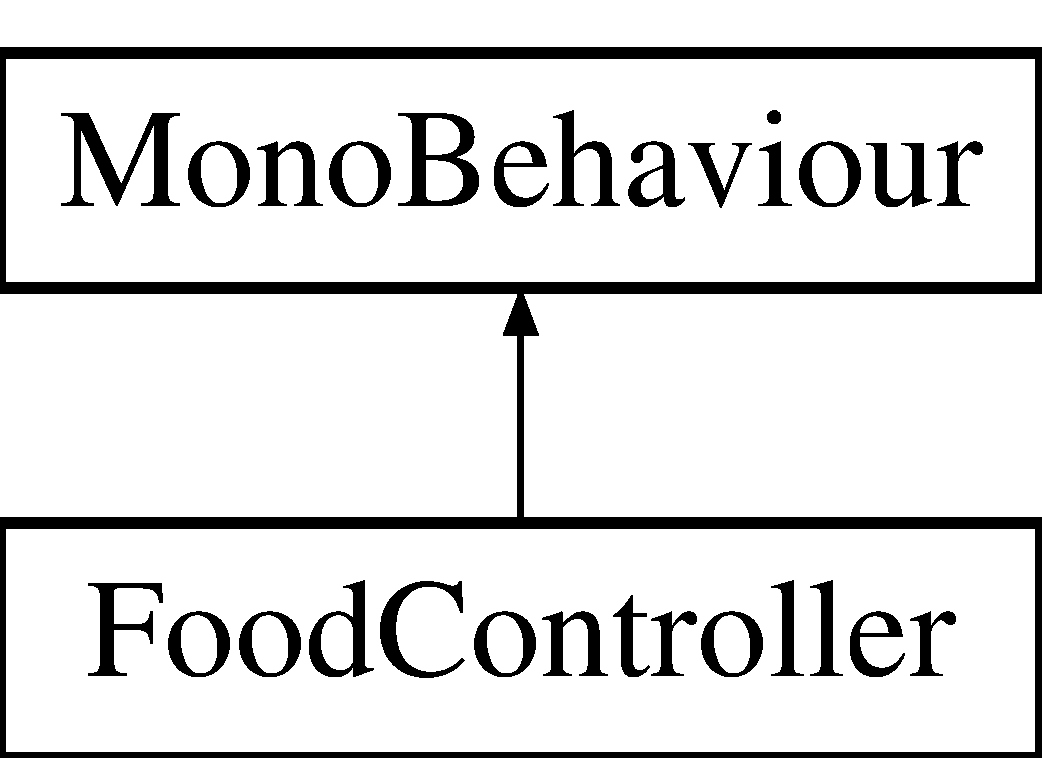
\includegraphics[height=2.000000cm]{class_food_controller}
\end{center}
\end{figure}
\subsection*{Public Types}
\begin{DoxyCompactItemize}
\item 
enum {\bfseries Movements} \{ {\bfseries Static}, 
{\bfseries Horizontal}, 
{\bfseries Vertical}, 
{\bfseries Random}
 \}\hypertarget{class_food_controller_ad3c2e51ce55236ad80384113f1593c79}{}\label{class_food_controller_ad3c2e51ce55236ad80384113f1593c79}

\end{DoxyCompactItemize}
\subsection*{Public Member Functions}
\begin{DoxyCompactItemize}
\item 
void \hyperlink{class_food_controller_a9f0f153ce5e90b4e081f4d903cf17808}{set\+Max\+Food\+Count} (string name, int count)
\begin{DoxyCompactList}\small\item\em Sets the max food count for the specified food type Can be called by Player \hyperlink{class_ability}{Ability} code \end{DoxyCompactList}\item 
int \hyperlink{class_food_controller_af9fcb378c2333de7796093ef368bfd93}{get\+Max\+Food\+Count} (string name)
\begin{DoxyCompactList}\small\item\em Gets the max food count for the specified food type Can be called by Player \hyperlink{class_ability}{Ability} code \end{DoxyCompactList}\item 
void \hyperlink{class_food_controller_ae118c67950b39a9b3aaa8e15f027a37b}{set\+Food\+Spawn\+Weight} (string name, float weight)
\begin{DoxyCompactList}\small\item\em Sets the food spawn probability weight for the specified food type Can be called by Player \hyperlink{class_ability}{Ability} code \end{DoxyCompactList}\item 
float \hyperlink{class_food_controller_aa210ae3e7b1cc83ba3dab4a36970e19f}{get\+Food\+Spawn\+Weight} (string name)
\begin{DoxyCompactList}\small\item\em Gets the food spawn probability weight for the specified food type Can be called by Player \hyperlink{class_ability}{Ability} code \end{DoxyCompactList}\item 
void \hyperlink{class_food_controller_a33196e4fa774e489de86cedaff452e83}{set\+Difficulty} (int level)
\begin{DoxyCompactList}\small\item\em Changes food spawning difficulty Can be called by \hyperlink{class_level_controller}{Level\+Controller} to change difficulty of the game \end{DoxyCompactList}\end{DoxyCompactItemize}
\subsection*{Public Attributes}
\begin{DoxyCompactItemize}
\item 
Sprite\mbox{[}$\,$\mbox{]} {\bfseries Food\+Sprites}\hypertarget{class_food_controller_a057095438030110578a6670576c6fa43}{}\label{class_food_controller_a057095438030110578a6670576c6fa43}

\end{DoxyCompactItemize}
\subsection*{Properties}
\begin{DoxyCompactItemize}
\item 
string\mbox{[}$\,$\mbox{]} {\bfseries Food\+Names}\hspace{0.3cm}{\ttfamily  \mbox{[}get\mbox{]}}\hypertarget{class_food_controller_a5780c78529b71e8dc914cff2963569b5}{}\label{class_food_controller_a5780c78529b71e8dc914cff2963569b5}

\item 
Dictionary$<$ string, int $>$ {\bfseries Food\+Values}\hspace{0.3cm}{\ttfamily  \mbox{[}get\mbox{]}}\hypertarget{class_food_controller_a4440f445f989fec97ae4ceee2ffbd841}{}\label{class_food_controller_a4440f445f989fec97ae4ceee2ffbd841}

\item 
Dictionary$<$ string, int $>$ {\bfseries Max\+Food\+Counts}\hspace{0.3cm}{\ttfamily  \mbox{[}get\mbox{]}}\hypertarget{class_food_controller_ab1af49799b84e19e2be274d9c5b149a4}{}\label{class_food_controller_ab1af49799b84e19e2be274d9c5b149a4}

\item 
Dictionary$<$ string, float $>$ {\bfseries Food\+Spawn\+Weights}\hspace{0.3cm}{\ttfamily  \mbox{[}get\mbox{]}}\hypertarget{class_food_controller_a41c8e47c4b31ac4de5f31599aeed0e36}{}\label{class_food_controller_a41c8e47c4b31ac4de5f31599aeed0e36}

\item 
Movements \hyperlink{class_food_controller_a345844b04406827705d89526d92a246d}{Food\+Movement}\hspace{0.3cm}{\ttfamily  \mbox{[}set\mbox{]}}
\begin{DoxyCompactList}\small\item\em Property to set food movement mode. (May not actually need this?) \end{DoxyCompactList}\end{DoxyCompactItemize}


\subsection{Detailed Description}
Script attached to \hyperlink{class_food_controller}{Food\+Controller} object that controls behavior such as food spawning, and food movement. 



\subsection{Member Function Documentation}
\index{Food\+Controller@{Food\+Controller}!get\+Food\+Spawn\+Weight@{get\+Food\+Spawn\+Weight}}
\index{get\+Food\+Spawn\+Weight@{get\+Food\+Spawn\+Weight}!Food\+Controller@{Food\+Controller}}
\subsubsection[{\texorpdfstring{get\+Food\+Spawn\+Weight(string name)}{getFoodSpawnWeight(string name)}}]{\setlength{\rightskip}{0pt plus 5cm}float Food\+Controller.\+get\+Food\+Spawn\+Weight (
\begin{DoxyParamCaption}
\item[{string}]{name}
\end{DoxyParamCaption}
)}\hypertarget{class_food_controller_aa210ae3e7b1cc83ba3dab4a36970e19f}{}\label{class_food_controller_aa210ae3e7b1cc83ba3dab4a36970e19f}


Gets the food spawn probability weight for the specified food type Can be called by Player \hyperlink{class_ability}{Ability} code 


\begin{DoxyParams}{Parameters}
{\em name} & \hyperlink{class_food}{Food} type to get spawn probability weight for\\
\hline
\end{DoxyParams}
\begin{DoxyReturn}{Returns}

\end{DoxyReturn}
\index{Food\+Controller@{Food\+Controller}!get\+Max\+Food\+Count@{get\+Max\+Food\+Count}}
\index{get\+Max\+Food\+Count@{get\+Max\+Food\+Count}!Food\+Controller@{Food\+Controller}}
\subsubsection[{\texorpdfstring{get\+Max\+Food\+Count(string name)}{getMaxFoodCount(string name)}}]{\setlength{\rightskip}{0pt plus 5cm}int Food\+Controller.\+get\+Max\+Food\+Count (
\begin{DoxyParamCaption}
\item[{string}]{name}
\end{DoxyParamCaption}
)}\hypertarget{class_food_controller_af9fcb378c2333de7796093ef368bfd93}{}\label{class_food_controller_af9fcb378c2333de7796093ef368bfd93}


Gets the max food count for the specified food type Can be called by Player \hyperlink{class_ability}{Ability} code 


\begin{DoxyParams}{Parameters}
{\em name} & \hyperlink{class_food}{Food} type to get count for\\
\hline
\end{DoxyParams}
\begin{DoxyReturn}{Returns}

\end{DoxyReturn}
\index{Food\+Controller@{Food\+Controller}!set\+Difficulty@{set\+Difficulty}}
\index{set\+Difficulty@{set\+Difficulty}!Food\+Controller@{Food\+Controller}}
\subsubsection[{\texorpdfstring{set\+Difficulty(int level)}{setDifficulty(int level)}}]{\setlength{\rightskip}{0pt plus 5cm}void Food\+Controller.\+set\+Difficulty (
\begin{DoxyParamCaption}
\item[{int}]{level}
\end{DoxyParamCaption}
)}\hypertarget{class_food_controller_a33196e4fa774e489de86cedaff452e83}{}\label{class_food_controller_a33196e4fa774e489de86cedaff452e83}


Changes food spawning difficulty Can be called by \hyperlink{class_level_controller}{Level\+Controller} to change difficulty of the game 


\begin{DoxyParams}{Parameters}
{\em level} & \\
\hline
\end{DoxyParams}
\index{Food\+Controller@{Food\+Controller}!set\+Food\+Spawn\+Weight@{set\+Food\+Spawn\+Weight}}
\index{set\+Food\+Spawn\+Weight@{set\+Food\+Spawn\+Weight}!Food\+Controller@{Food\+Controller}}
\subsubsection[{\texorpdfstring{set\+Food\+Spawn\+Weight(string name, float weight)}{setFoodSpawnWeight(string name, float weight)}}]{\setlength{\rightskip}{0pt plus 5cm}void Food\+Controller.\+set\+Food\+Spawn\+Weight (
\begin{DoxyParamCaption}
\item[{string}]{name, }
\item[{float}]{weight}
\end{DoxyParamCaption}
)}\hypertarget{class_food_controller_ae118c67950b39a9b3aaa8e15f027a37b}{}\label{class_food_controller_ae118c67950b39a9b3aaa8e15f027a37b}


Sets the food spawn probability weight for the specified food type Can be called by Player \hyperlink{class_ability}{Ability} code 


\begin{DoxyParams}{Parameters}
{\em name} & \\
\hline
{\em weight} & \\
\hline
\end{DoxyParams}
\index{Food\+Controller@{Food\+Controller}!set\+Max\+Food\+Count@{set\+Max\+Food\+Count}}
\index{set\+Max\+Food\+Count@{set\+Max\+Food\+Count}!Food\+Controller@{Food\+Controller}}
\subsubsection[{\texorpdfstring{set\+Max\+Food\+Count(string name, int count)}{setMaxFoodCount(string name, int count)}}]{\setlength{\rightskip}{0pt plus 5cm}void Food\+Controller.\+set\+Max\+Food\+Count (
\begin{DoxyParamCaption}
\item[{string}]{name, }
\item[{int}]{count}
\end{DoxyParamCaption}
)}\hypertarget{class_food_controller_a9f0f153ce5e90b4e081f4d903cf17808}{}\label{class_food_controller_a9f0f153ce5e90b4e081f4d903cf17808}


Sets the max food count for the specified food type Can be called by Player \hyperlink{class_ability}{Ability} code 


\begin{DoxyParams}{Parameters}
{\em name} & Name of food\\
\hline
{\em count} & Max count to set to\\
\hline
\end{DoxyParams}


\subsection{Property Documentation}
\index{Food\+Controller@{Food\+Controller}!Food\+Movement@{Food\+Movement}}
\index{Food\+Movement@{Food\+Movement}!Food\+Controller@{Food\+Controller}}
\subsubsection[{\texorpdfstring{Food\+Movement}{FoodMovement}}]{\setlength{\rightskip}{0pt plus 5cm}Movements Food\+Controller.\+Food\+Movement\hspace{0.3cm}{\ttfamily [set]}}\hypertarget{class_food_controller_a345844b04406827705d89526d92a246d}{}\label{class_food_controller_a345844b04406827705d89526d92a246d}


Property to set food movement mode. (May not actually need this?) 



The documentation for this class was generated from the following file\+:\begin{DoxyCompactItemize}
\item 
Assets/\+Scripts/Food\+Controller.\+cs\end{DoxyCompactItemize}

\hypertarget{class_mouse}{}\section{Mouse Class Reference}
\label{class_mouse}\index{Mouse@{Mouse}}


Script class that controls behaviour of the mouse. Keeps track of mouses status such as weight, happiness, level, and attributes that can be set by player abilities\+: (immunity, leptin\+Deficiency, fearless)  


Inheritance diagram for Mouse\+:\begin{figure}[H]
\begin{center}
\leavevmode
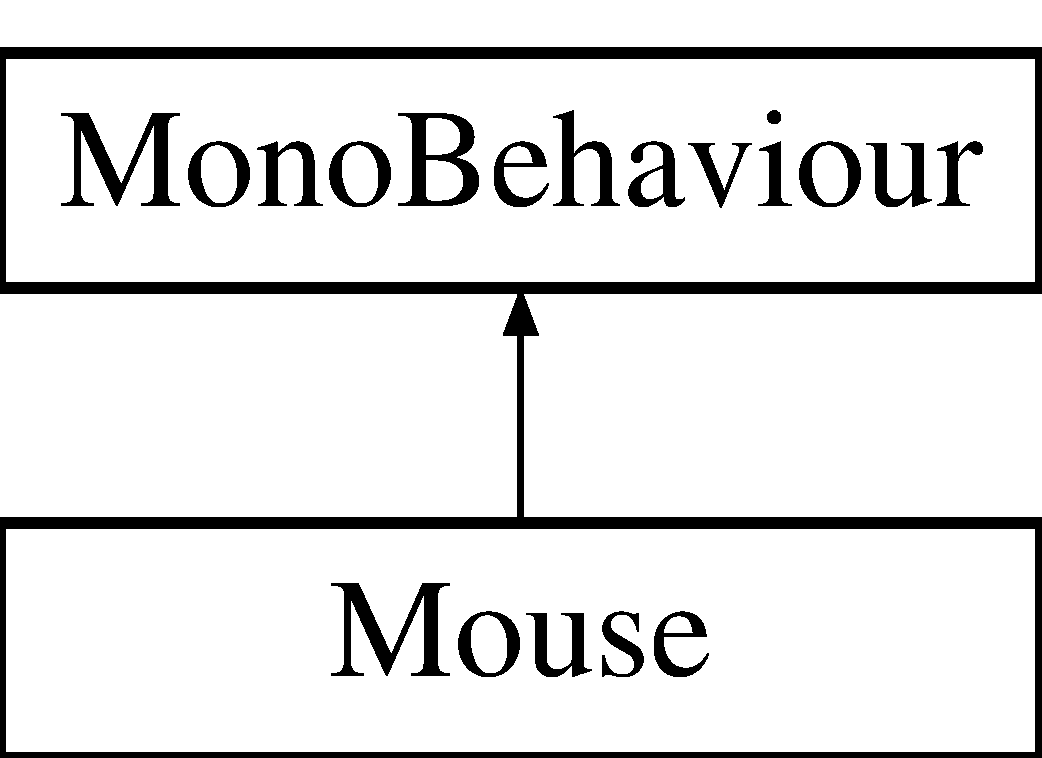
\includegraphics[height=2.000000cm]{class_mouse}
\end{center}
\end{figure}
\subsection*{Public Attributes}
\begin{DoxyCompactItemize}
\item 
Sprite\mbox{[}$\,$\mbox{]} {\bfseries Level\+Sprites} = new Sprite\mbox{[}11\mbox{]}\hypertarget{class_mouse_a215f93e37bb5d78b3890c79507461f1f}{}\label{class_mouse_a215f93e37bb5d78b3890c79507461f1f}

\item 
Sprite\mbox{[}$\,$\mbox{]} {\bfseries Happiness\+Sprites} = new Sprite\mbox{[}5\mbox{]}\hypertarget{class_mouse_a4c4febebe798e39398129c308a3b7c70}{}\label{class_mouse_a4c4febebe798e39398129c308a3b7c70}

\end{DoxyCompactItemize}
\subsection*{Properties}
\begin{DoxyCompactItemize}
\item 
int \hyperlink{class_mouse_add4f90aa1a1e81b981a6b2dfdb0c9e24}{Weight}\hspace{0.3cm}{\ttfamily  \mbox{[}get, set\mbox{]}}
\begin{DoxyCompactList}\small\item\em Property to get mouse weight. Read only. \end{DoxyCompactList}\item 
int \hyperlink{class_mouse_a76debda38af30b4b2249757bc316f66e}{Level}\hspace{0.3cm}{\ttfamily  \mbox{[}get\mbox{]}}
\begin{DoxyCompactList}\small\item\em Property to get mouse level. Read only. \end{DoxyCompactList}\item 
int {\bfseries Happiness}\hspace{0.3cm}{\ttfamily  \mbox{[}get, set\mbox{]}}\hypertarget{class_mouse_a91cb125845991ce20246753f7eef2b8e}{}\label{class_mouse_a91cb125845991ce20246753f7eef2b8e}

\item 
bool \hyperlink{class_mouse_a7916f98be8b4afcd422794bbf8994e25}{Immunity}\hspace{0.3cm}{\ttfamily  \mbox{[}get, set\mbox{]}}
\begin{DoxyCompactList}\small\item\em Property to get and set mouse immunity Can be called by Player \hyperlink{class_ability}{Ability} code \end{DoxyCompactList}\item 
int \hyperlink{class_mouse_a58afb42b0fa0f4d9fb30795d68a86b82}{Growth\+Ability}\hspace{0.3cm}{\ttfamily  \mbox{[}get, set\mbox{]}}
\begin{DoxyCompactList}\small\item\em Property to get and set mouse growth ability (leptin deficiency) Can be called by Player \hyperlink{class_ability}{Ability} code \end{DoxyCompactList}\item 
bool \hyperlink{class_mouse_aa866c3f02e0e310895d8e5ef4bca6db5}{Fearless}\hspace{0.3cm}{\ttfamily  \mbox{[}get, set\mbox{]}}
\begin{DoxyCompactList}\small\item\em Property to get and set mouse fearless(ness) Can be called by Player \hyperlink{class_ability}{Ability} code \end{DoxyCompactList}\item 
bool \hyperlink{class_mouse_a4bdbd8793c98c76e0ed8b00717d34325}{Offscreen}\hspace{0.3cm}{\ttfamily  \mbox{[}get, set\mbox{]}}
\begin{DoxyCompactList}\small\item\em Property to get and set whether the mouse is off-\/screen Can be called by Player \hyperlink{class_ability}{Ability} code \end{DoxyCompactList}\end{DoxyCompactItemize}


\subsection{Detailed Description}
Script class that controls behaviour of the mouse. Keeps track of mouses status such as weight, happiness, level, and attributes that can be set by player abilities\+: (immunity, leptin\+Deficiency, fearless) 



\subsection{Property Documentation}
\index{Mouse@{Mouse}!Fearless@{Fearless}}
\index{Fearless@{Fearless}!Mouse@{Mouse}}
\subsubsection[{\texorpdfstring{Fearless}{Fearless}}]{\setlength{\rightskip}{0pt plus 5cm}bool Mouse.\+Fearless\hspace{0.3cm}{\ttfamily [get]}, {\ttfamily [set]}}\hypertarget{class_mouse_aa866c3f02e0e310895d8e5ef4bca6db5}{}\label{class_mouse_aa866c3f02e0e310895d8e5ef4bca6db5}


Property to get and set mouse fearless(ness) Can be called by Player \hyperlink{class_ability}{Ability} code 

\index{Mouse@{Mouse}!Growth\+Ability@{Growth\+Ability}}
\index{Growth\+Ability@{Growth\+Ability}!Mouse@{Mouse}}
\subsubsection[{\texorpdfstring{Growth\+Ability}{GrowthAbility}}]{\setlength{\rightskip}{0pt plus 5cm}int Mouse.\+Growth\+Ability\hspace{0.3cm}{\ttfamily [get]}, {\ttfamily [set]}}\hypertarget{class_mouse_a58afb42b0fa0f4d9fb30795d68a86b82}{}\label{class_mouse_a58afb42b0fa0f4d9fb30795d68a86b82}


Property to get and set mouse growth ability (leptin deficiency) Can be called by Player \hyperlink{class_ability}{Ability} code 

\index{Mouse@{Mouse}!Immunity@{Immunity}}
\index{Immunity@{Immunity}!Mouse@{Mouse}}
\subsubsection[{\texorpdfstring{Immunity}{Immunity}}]{\setlength{\rightskip}{0pt plus 5cm}bool Mouse.\+Immunity\hspace{0.3cm}{\ttfamily [get]}, {\ttfamily [set]}}\hypertarget{class_mouse_a7916f98be8b4afcd422794bbf8994e25}{}\label{class_mouse_a7916f98be8b4afcd422794bbf8994e25}


Property to get and set mouse immunity Can be called by Player \hyperlink{class_ability}{Ability} code 

\index{Mouse@{Mouse}!Level@{Level}}
\index{Level@{Level}!Mouse@{Mouse}}
\subsubsection[{\texorpdfstring{Level}{Level}}]{\setlength{\rightskip}{0pt plus 5cm}int Mouse.\+Level\hspace{0.3cm}{\ttfamily [get]}}\hypertarget{class_mouse_a76debda38af30b4b2249757bc316f66e}{}\label{class_mouse_a76debda38af30b4b2249757bc316f66e}


Property to get mouse level. Read only. 

\index{Mouse@{Mouse}!Offscreen@{Offscreen}}
\index{Offscreen@{Offscreen}!Mouse@{Mouse}}
\subsubsection[{\texorpdfstring{Offscreen}{Offscreen}}]{\setlength{\rightskip}{0pt plus 5cm}bool Mouse.\+Offscreen\hspace{0.3cm}{\ttfamily [get]}, {\ttfamily [set]}}\hypertarget{class_mouse_a4bdbd8793c98c76e0ed8b00717d34325}{}\label{class_mouse_a4bdbd8793c98c76e0ed8b00717d34325}


Property to get and set whether the mouse is off-\/screen Can be called by Player \hyperlink{class_ability}{Ability} code 

\index{Mouse@{Mouse}!Weight@{Weight}}
\index{Weight@{Weight}!Mouse@{Mouse}}
\subsubsection[{\texorpdfstring{Weight}{Weight}}]{\setlength{\rightskip}{0pt plus 5cm}int Mouse.\+Weight\hspace{0.3cm}{\ttfamily [get]}, {\ttfamily [set]}}\hypertarget{class_mouse_add4f90aa1a1e81b981a6b2dfdb0c9e24}{}\label{class_mouse_add4f90aa1a1e81b981a6b2dfdb0c9e24}


Property to get mouse weight. Read only. 



The documentation for this class was generated from the following file\+:\begin{DoxyCompactItemize}
\item 
Assets/\+Scripts/Mouse.\+cs\end{DoxyCompactItemize}

\hypertarget{class_object_pool}{}\section{Object\+Pool Class Reference}
\label{class_object_pool}\index{Object\+Pool@{Object\+Pool}}


Generic class for handling object pooling. The type of game object to pool can be specified by assigning the public member obj in the inspector panel. Keeps track of active objects in the pool. Has methods to get object from pool and return object to the pool. Pool is maintained as a list and can grow dynamically.  


Inheritance diagram for Object\+Pool\+:\begin{figure}[H]
\begin{center}
\leavevmode
\includegraphics[height=2.000000cm]{class_object_pool}
\end{center}
\end{figure}
\subsection*{Public Member Functions}
\begin{DoxyCompactItemize}
\item 
Game\+Object \hyperlink{class_object_pool_a1a2f42245b2acfef316e203e6a88c7f2}{get\+Obj} ()
\begin{DoxyCompactList}\small\item\em Gets an object from the pool. If the pool is empty, instantiates a new object and dynamically grows the pool. \end{DoxyCompactList}\item 
void \hyperlink{class_object_pool_a61d15dbf443949f7a0b59031c6a8d2e4}{return\+Obj} (Game\+Object obj)
\begin{DoxyCompactList}\small\item\em Returns a specified object to the pool. To be called by \hyperlink{class_pool_member_a6f883eaed133e4b288a3847aea3ff33a}{Pool\+Member\+::\+Deactivate()} \end{DoxyCompactList}\end{DoxyCompactItemize}
\subsection*{Properties}
\begin{DoxyCompactItemize}
\item 
int \hyperlink{class_object_pool_a60d15ca98c4df8f2698431d968570eac}{Active\+Objects}\hspace{0.3cm}{\ttfamily  \mbox{[}get\mbox{]}}
\begin{DoxyCompactList}\small\item\em Gets the number of active objects that were released from the pool. \end{DoxyCompactList}\item 
Game\+Object \hyperlink{class_object_pool_aff4a0bc1bec2c6575f8df0f7e9fd62f4}{pool\+Object}\hspace{0.3cm}{\ttfamily  \mbox{[}get, set\mbox{]}}
\begin{DoxyCompactList}\small\item\em Property to get and set object of the pool \end{DoxyCompactList}\end{DoxyCompactItemize}


\subsection{Detailed Description}
Generic class for handling object pooling. The type of game object to pool can be specified by assigning the public member obj in the inspector panel. Keeps track of active objects in the pool. Has methods to get object from pool and return object to the pool. Pool is maintained as a list and can grow dynamically. 



\subsection{Member Function Documentation}
\index{Object\+Pool@{Object\+Pool}!get\+Obj@{get\+Obj}}
\index{get\+Obj@{get\+Obj}!Object\+Pool@{Object\+Pool}}
\subsubsection[{\texorpdfstring{get\+Obj()}{getObj()}}]{\setlength{\rightskip}{0pt plus 5cm}Game\+Object Object\+Pool.\+get\+Obj (
\begin{DoxyParamCaption}
{}
\end{DoxyParamCaption}
)}\hypertarget{class_object_pool_a1a2f42245b2acfef316e203e6a88c7f2}{}\label{class_object_pool_a1a2f42245b2acfef316e203e6a88c7f2}


Gets an object from the pool. If the pool is empty, instantiates a new object and dynamically grows the pool. 

\begin{DoxyReturn}{Returns}

\end{DoxyReturn}
\index{Object\+Pool@{Object\+Pool}!return\+Obj@{return\+Obj}}
\index{return\+Obj@{return\+Obj}!Object\+Pool@{Object\+Pool}}
\subsubsection[{\texorpdfstring{return\+Obj(\+Game\+Object obj)}{returnObj(GameObject obj)}}]{\setlength{\rightskip}{0pt plus 5cm}void Object\+Pool.\+return\+Obj (
\begin{DoxyParamCaption}
\item[{Game\+Object}]{obj}
\end{DoxyParamCaption}
)}\hypertarget{class_object_pool_a61d15dbf443949f7a0b59031c6a8d2e4}{}\label{class_object_pool_a61d15dbf443949f7a0b59031c6a8d2e4}


Returns a specified object to the pool. To be called by \hyperlink{class_pool_member_a6f883eaed133e4b288a3847aea3ff33a}{Pool\+Member\+::\+Deactivate()} 


\begin{DoxyParams}{Parameters}
{\em obj} & \\
\hline
\end{DoxyParams}


\subsection{Property Documentation}
\index{Object\+Pool@{Object\+Pool}!Active\+Objects@{Active\+Objects}}
\index{Active\+Objects@{Active\+Objects}!Object\+Pool@{Object\+Pool}}
\subsubsection[{\texorpdfstring{Active\+Objects}{ActiveObjects}}]{\setlength{\rightskip}{0pt plus 5cm}int Object\+Pool.\+Active\+Objects\hspace{0.3cm}{\ttfamily [get]}}\hypertarget{class_object_pool_a60d15ca98c4df8f2698431d968570eac}{}\label{class_object_pool_a60d15ca98c4df8f2698431d968570eac}


Gets the number of active objects that were released from the pool. 

\begin{DoxyReturn}{Returns}

\end{DoxyReturn}
\index{Object\+Pool@{Object\+Pool}!pool\+Object@{pool\+Object}}
\index{pool\+Object@{pool\+Object}!Object\+Pool@{Object\+Pool}}
\subsubsection[{\texorpdfstring{pool\+Object}{poolObject}}]{\setlength{\rightskip}{0pt plus 5cm}Game\+Object Object\+Pool.\+pool\+Object\hspace{0.3cm}{\ttfamily [get]}, {\ttfamily [set]}}\hypertarget{class_object_pool_aff4a0bc1bec2c6575f8df0f7e9fd62f4}{}\label{class_object_pool_aff4a0bc1bec2c6575f8df0f7e9fd62f4}


Property to get and set object of the pool 



The documentation for this class was generated from the following file\+:\begin{DoxyCompactItemize}
\item 
Assets/\+Scripts/Object\+Pool.\+cs\end{DoxyCompactItemize}

\hypertarget{class_pool_member}{}\section{Pool\+Member Class Reference}
\label{class_pool_member}\index{Pool\+Member@{Pool\+Member}}


Script that is attached to members of an object pool when they are first instantiated. Allows object to keep track of the pool they belong to and be deactivated and returned to that pool.  


Inheritance diagram for Pool\+Member\+:\begin{figure}[H]
\begin{center}
\leavevmode
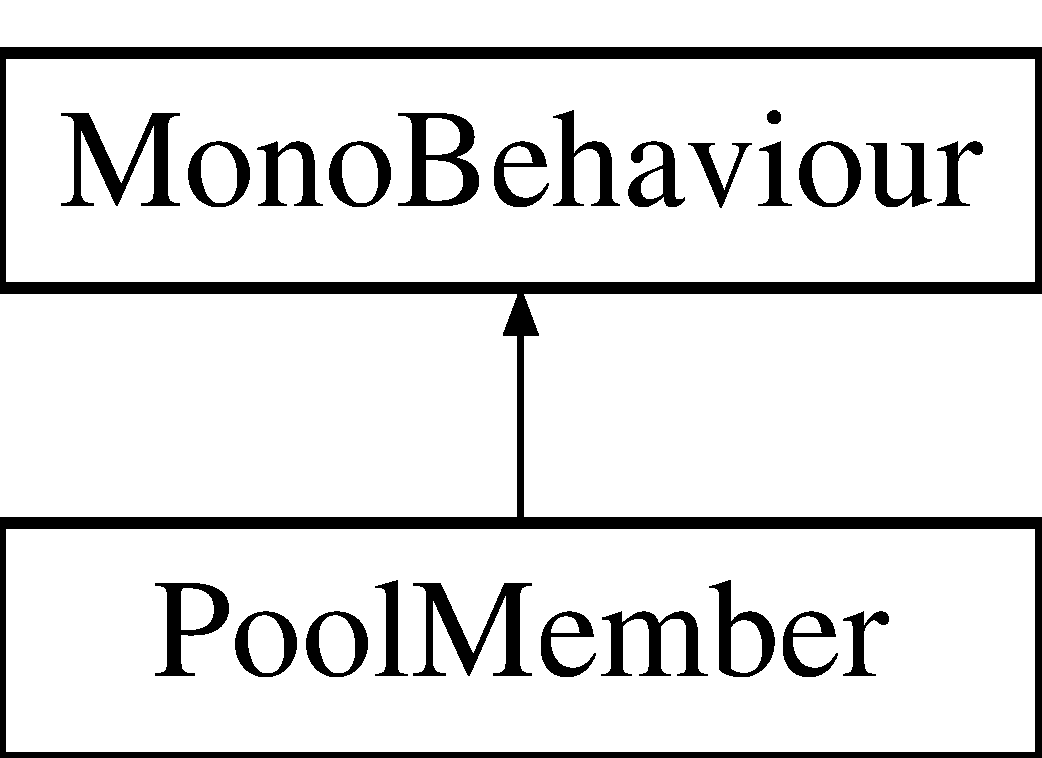
\includegraphics[height=2.000000cm]{class_pool_member}
\end{center}
\end{figure}
\subsection*{Public Member Functions}
\begin{DoxyCompactItemize}
\item 
void \hyperlink{class_pool_member_a6f883eaed133e4b288a3847aea3ff33a}{Deactivate} ()
\begin{DoxyCompactList}\small\item\em Deactivates and returns the object to its pool \end{DoxyCompactList}\item 
void {\bfseries set\+Pool} (\hyperlink{class_object_pool}{Object\+Pool} pool)\hypertarget{class_pool_member_aa20f1ac6e12b3d7d3b6f71d49e0cd1af}{}\label{class_pool_member_aa20f1ac6e12b3d7d3b6f71d49e0cd1af}

\end{DoxyCompactItemize}


\subsection{Detailed Description}
Script that is attached to members of an object pool when they are first instantiated. Allows object to keep track of the pool they belong to and be deactivated and returned to that pool. 



\subsection{Member Function Documentation}
\index{Pool\+Member@{Pool\+Member}!Deactivate@{Deactivate}}
\index{Deactivate@{Deactivate}!Pool\+Member@{Pool\+Member}}
\subsubsection[{\texorpdfstring{Deactivate()}{Deactivate()}}]{\setlength{\rightskip}{0pt plus 5cm}void Pool\+Member.\+Deactivate (
\begin{DoxyParamCaption}
{}
\end{DoxyParamCaption}
)}\hypertarget{class_pool_member_a6f883eaed133e4b288a3847aea3ff33a}{}\label{class_pool_member_a6f883eaed133e4b288a3847aea3ff33a}


Deactivates and returns the object to its pool 



The documentation for this class was generated from the following file\+:\begin{DoxyCompactItemize}
\item 
Assets/\+Scripts/Pool\+Member.\+cs\end{DoxyCompactItemize}

\hypertarget{class_touch_test}{}\section{Touch\+Test Class Reference}
\label{class_touch_test}\index{Touch\+Test@{Touch\+Test}}
Inheritance diagram for Touch\+Test\+:\begin{figure}[H]
\begin{center}
\leavevmode
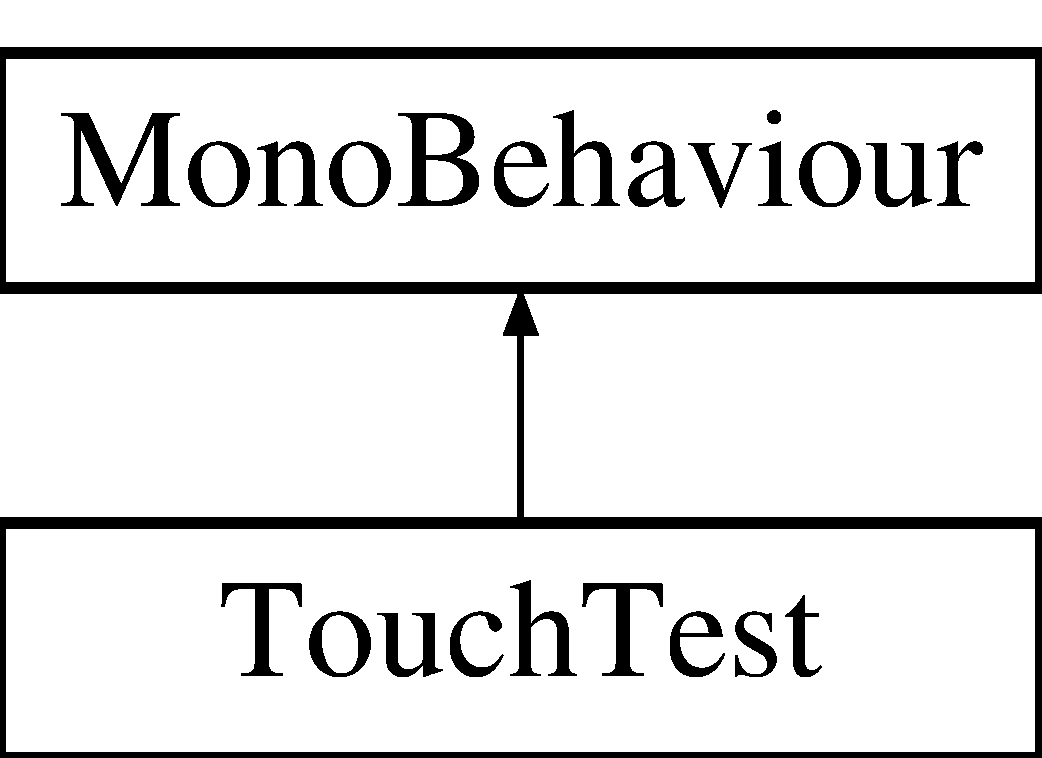
\includegraphics[height=2.000000cm]{class_touch_test}
\end{center}
\end{figure}


The documentation for this class was generated from the following file\+:\begin{DoxyCompactItemize}
\item 
Assets/\+Scripts/Touch\+Test.\+cs\end{DoxyCompactItemize}

%--- End generated contents ---

% Index
\backmatter
\newpage
\phantomsection
\clearemptydoublepage
\addcontentsline{toc}{chapter}{Index}
\printindex

\end{document}
